\label{sec:io}
There are multiple ways a computer can communicate with its peripheral devices.
The most used techniques are Memory-Mapped I/O (MMIO) and Port-Mapped I/O
(PMIO). Port-Mapped I/O is an older method of accessing peripherals, and is much
more common in consumer computers with Intel or AMD CPUs\cite{intelmanual}.\\
PMIO requires the processor to have additional pins and special instructions,
just for communication with I/O devices. I/O devices have a specified port
number, which the processor uses to identify and communicate with the device,
much like an address.
For example, Intel x86 processors might be polling\footnote{Polling refers to
the activity where a CPU periodically samples the status of an external device}
a keyboard using the special \texttt{in} instruction, specifying the predefined
keyboard status ID \texttt{0x60}, then reading from keyboard data, with ID
\texttt{0x64}\cite{intel:pch}\cite{osdev:io_ports}:
\begin{lstlisting}[language={[x86masm]Assembler}]
_wait:
  in  al, 64H ; Read keyboard status
  and al, 1   ; Check if ready
  jz  _wait
  in  al, 60H ; Read keyboard data
\end{lstlisting}
Besides the added circuitry in the processor, port-mapped I/O are fairly
simple to implement for chip manufacturers, and easy to use for programmers.
They have their own special instructions,
and they do not share memory space, which prevents confusion about
memory segmenting.
However, PMIO approach is very limited to only \texttt{in} and \texttt{out}
instructions, reading only a few bytes at a time into the EAX register, as well
as a limited port numbers for the devices.\cite{intelmanual}\\

Memory-Mapped I/O is commonly used by RISC architectures. In MMIO,
communication with the peripherals happens over the same address bus as the
memory, so that memory and I/O communication share address space. This means
that when a processor, that uses MMIO, wants to access a peripheral, it uses a
memory address for communication.\\
The advantage of memory-mapped I/O is that the method uses already existing
memory bus lanes for communication, unlike the port implementation. However,
since the memory is shared with peripherals, and these addresses are not
maintained by the processor, additional logic has to be created in the
memory-management unit (discussed in the next section). However, PMIO is very limited to the simple \texttt{in
/ out} instructions, as well as a hardware-limited device allocation, whereas
MMIO is much more free with device "address" allocation. Due to these reasons,
memory-mapped I/O is becoming increasingly popular, even on modern x86
hardware\cite{osdev:io_ports}.\\
MIPS initially sees Input/Output (IO) devices as a set of special-purpose registers. These
special registers are the processors only way of communicating with a given
device.\\
For every device, there 3 types of
registers\cite{cs_uwm:memory_mapped_io}\cite{imgtec:pra}:
\begin{itemize}
	\item \texttt{Status registers}\\
	Provide information about the underlying device. These registers are
	read-only for the CPU.

	\item \texttt{Control registers}\\
	Used to communicate and control the device. These registers are
	writeable for the CPU, but may not always be readable.

	\item \texttt{Data registers}\\
	Used for the actual data-transport. For example, the latest key pressed
	on the keyboard might be stored in this register.
\end{itemize}

On MIPS32, in the memory, these registers have allocated 4 bytes each, and are
always located sequentially in the memory. Figure \ref{fig:io_registers} shows
the actual bit-allocation in the register.
\begin{figure}[H]
	\centering
	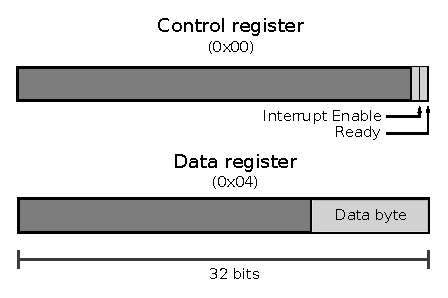
\includegraphics[scale=1]{io/io_registers.eps}
	\caption{Set of memory mapped I/O registers\cite{imgtec:pra}}
	\label{fig:io_registers}
\end{figure}

When a device is detected, the memory-management unit will allocate an address
for the device, notifying both the CPU and the device of these newly allocated registers.
From now on, it is up to the driver to interface with the devices.\\
Depending on the type of the IO device, the device can be represented from a
few registers to dozens. For example, a mouse or a keyboard only transmits few
bytes of information at a time, needing only a few registers, while graphic
adaptors or disk drives might need more\cite{cs_uwm:memory_mapped_io}.\\
These special-purpose registers are located in the memory, mapped to a certain
segment. A device controller maintains a list of these registers, and maps new
devices to the memory.\cite{britton:mips}\\
On MIPS32, the highest 64 kilobytes (\texttt{0xffff0000 - 0xffffffff}) in the
available memory are used for mapping these special registers\cite{cs_uwm:memory_mapped_io}.
The memory mapping the IO area must not be cached, as it can cause major problems
for the caches, and heavy delays due to many cache-misses\cite{see_mips_run}.\\
However, it is obvious that IO registers can be very inconvenient for larger and
fast data-transfer, due to the very limited register size. To dodge this
bottleneck, memory controllers are implemented to give IO devices direct access
to larger parts of the main memory, without the need of going through the CPU first.

\subsection{Direct Memory Access}
Direct Memory Access controllers, also called DMA controllers, allow certain
hardware to access the main memory independently of the CPU.
In MIPS, this feature is built-in in the MMU.\\
Larger transfers between hardware and the memory is usually initiated through
the device registers, where the CPU sets up the MMU and communicates the target
address. Then, the IO device is free to read and write in the target address.
When the peripheral is finished with its actions on the memory, it will usually
notify the CPU using an interrupt, having the processor taking care of the rest.\\
Direct Memory Access is often utilized by peripherals with heavy IO use, such
as the storage drives, as well as network-, sound-, and graphics-cards.\\
Because KUDOS does not read large portions of data from its IO devices, nor is
there any DMA support in the current YAMS simulator, DMA will not be implemented.

\subsection{Detecting and mapping peripherals}
When a computer is turned on, or a new peripheral device is plugged in, the MIPS
processor and its MMU automatically map the device to a given address, allocating
the necessary IO registers. All this happens seamlessly and without the interaction
of the operating system. This is problematic, because the OS needs to know the
type of the device and the address of its memory mapped registers, amongst other
things. There is no real way to communicate this between the processor and the
operating system. To make matters worse, each processor has its own addresses
for the registers, and a slightly different configuration. On top of that, each
board has its own set of external components, busses and metadevices\cite{devicetree_spec}\cite{xillybus:devicetree}.
Instead of compiling a very specialized kernel for seemingly every configuration
of a System on a Chip (SoC), operating system and bootloader developers have
designed a specification \emph{devicetree}, which is used to describe system
hardware\cite{devicetree_spec}.\\
The devicetree specification can describe a lot of aspects of a hardware devices,
such as the interrupt number, size of the IO registers, even the device clock
speeds.\\
The Linux kernel also enjoys this devicetree specification, both for ARM and
MIPS architecuters\cite[\texttt{linux-4.6/arch/mips/boot/dts}]{linux}, reducing the time
and complexity of implementing a new board or a SoC.\\
In KUDOS, this data structure is unfortunatelly not used, because the hardware
it runs on is very limited, consisting almost only of simulated devices. As
a result of that, KUDOS looks at a predefined address for data structures
describing the devices, called the device descriptors.

\subsection{Device descriptors}
To detect and communicate with external devices, device descriptors are used.
A device descriptor is a data structure which, just like a devicetree, specifies
all the relevant information about the device, such as its type, name, register
addresses and so on. The format of the device descriptor is defined in Yet Another
MIPS Simulator, the current simulator used to run KUDOS. The same device descriptor
structure is defined in KUDOS, so that KUDOS can interface with the underlying
simulator, retrieving the relevant information.
The structure is defined in \texttt{kudos/drivers/mips32/arch.h}\cite{kudos} as:
\begin{lstlisting}[language=c]
typedef struct {
    uint32_t type;
    uint32_t io_area_base;
    uint32_t io_area_len;
    uint32_t irq;
    char vendor_string[8];

   /* Reserved area (unused). */
    uint32_t resv[2];
} io_descriptor_t;
\end{lstlisting}

Learning from the devicetree specification and the seasoned Linux developers,
it would probably be better with a more general method to describe system
hardware. However, to be compatible with KUDOS and not break it, we will use
this exact same interface with devices, although modifying its location in
memory slightly.


\subsection{Implementation}
Implementation of external devices requires a lot of new modules and features
in the simulator. The main issue is that we require to communicate with
events, not necessarily handled by the simulator.



\begin{figure}[H]
	\centering
	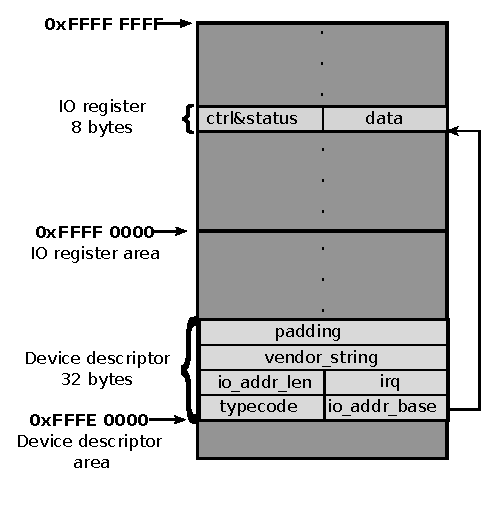
\includegraphics[scale=1]{io/io_memory_layout.eps}
	\caption{Memory layout of IO device descriptors and registers.}
	\label{fig:io_memory_layout}
\end{figure}


\subsection{Hardware Devices}
Naturally, we are going to need to implement some essential hardware devices
for KUDOS to use.\\
There are no definite specifications for how a hardware device must work.
Effectivelly, each manufacturer decides the specification of their devices
themselves. It is impossible for an operating system to keep track of all these
devices, and so, a special kind of interface, called a \texttt{driver},
is implemented and used for each device.\\
Most drivers are specific to certain devices, removing the subsequent complexity
for the communication with the device. This is also why certain devices refuse
to work in Linux, Windows or other OS, before the correct driver is installed.
\cite{microsoft:driver}\\
Lucky for us, we can define our own devices and its drivers -- that is,
we do not emulate an existing device, rather we define our own, with its own
set of magic numbers, IO registers etc.


\subsubsection{Shutdown device}
The first most important device is the shutdown-device, which turns off the
device (in our case, the simulator).
In KUDOS and YAMS, this device is implemented with only 1 data register, which
will trigger a shutdown, if a magic number \texttt{POWEROFF\_SHUTDOWN\_MAGIC} is
written to it\cite[drivers/metadev.h]{kudos}.\\
In the simulator, if the write-address is that of the shutdown device, and the
magic number is known, the global boolean variable \texttt{g\_finished} is
toggled, stopping the simulator.\\
Once again, to avoid unneccesarry compatibility breaks with YAMS, we will use
the same magic number.

\subsubsection{TTY device}

